% Generated from the public primitive catalog. Original Atlas drawing; Apache-2.0.
% Target: tdea-3key; view: overview
\documentclass[border=9pt]{standalone}
% Original Atlas figure theme. Apache-2.0; see the repository LICENSE.
\usepackage[T1]{fontenc}
\usepackage{lmodern}
\usepackage{amsmath,amssymb}
\usepackage{tikz}
\usetikzlibrary{arrows.meta,positioning,calc,fit,backgrounds,decorations.pathreplacing,matrix}
\definecolor{atlasInk}{HTML}{172235}
\definecolor{atlasTeal}{HTML}{0D7B7D}
\definecolor{atlasMuted}{HTML}{637278}
\definecolor{atlasFill}{HTML}{EAF4F2}
\definecolor{atlasLine}{HTML}{B6C8C7}
\tikzset{
  every picture/.style={line width=.65pt,draw=atlasInk,>=Latex},
  every node/.style={text=atlasInk,font=\sffamily\small},
  box/.style={draw,rounded corners=1.5pt,minimum height=.9cm,minimum width=1.6cm,align=center,inner sep=6pt,fill=white},
  accent/.style={box,draw=atlasTeal,fill=atlasFill},
  wire/.style={->,line width=.7pt},
  keywire/.style={wire,draw=atlasTeal,dashed},
  xor/.style={draw,circle,fill=white,inner sep=0pt,minimum size=.38cm},
  add/.style={draw,rectangle,fill=white,inner sep=0pt,minimum size=.38cm},
  note/.style={font=\sffamily\scriptsize,text=atlasMuted,align=center},
  phase/.style={font=\sffamily\small\bfseries,text=atlasTeal},
  group/.style={draw=atlasLine,dashed,rounded corners=2pt,inner sep=8pt}
}
\newcommand{\rotl}{\mathbin{\lll}}
\newcommand{\rotr}{\mathbin{\ggg}}
\newcommand{\kx}{\operatorname{Keccak}\!\text{-}\!f[1600]}

\newcommand{\AtlasKeyBits}{168}
\newcommand{\AtlasKeyWords}{5.25}
\newcommand{\AtlasRounds}{16}
\newcommand{\AtlasPriorRounds}{15}
\newcommand{\AtlasRoundKeys}{17}
\newcommand{\AtlasDoubleRounds}{8}
\newcommand{\AtlasSixRoundGroups}{2.6666666666666665}
\newcommand{\AtlasFLGroups}{1.6666666666666665}
\newcommand{\AtlasRoundStart}{8}
\newcommand{\AtlasBlockBits}{64}
\newcommand{\AtlasOutputBits}{d}
\newcommand{\AtlasStateBits}{8w}
\newcommand{\AtlasNonceBits}{v}
\newcommand{\AtlasCounterBits}{q}
\newcommand{\AtlasStreamBlockBits}{b}
\newcommand{\AtlasRate}{r}
\newcommand{\AtlasCapacity}{c}
\newcommand{\AtlasSteps}{N}
\newcommand{\AtlasLastStep}{N-1}
\newcommand{\AtlasWordBits}{w}
\newcommand{\AtlasHashWords}{h}
\newcommand{\AtlasFeedForward}{\boxplus}
\newcommand{\AtlasByteOrder}{big-endian}
\newcommand{\AtlasDomain}{01}
\newif\ifAtlasXof
\AtlasXoffalse
\begin{document}
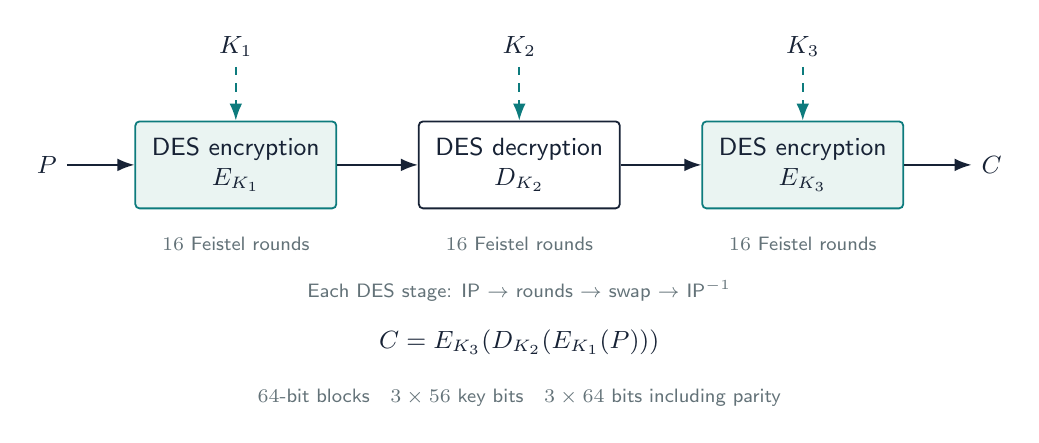
\begin{tikzpicture}
  \node (p) at (0,0) {$P$};
  \node[accent] (e1) at (2.4,0) {DES encryption\\$E_{K_1}$};
  \node[box] (d) at (6,0) {DES decryption\\$D_{K_2}$};
  \node[accent] (e2) at (9.6,0) {DES encryption\\$E_{K_3}$};
  \node (c) at (12,0) {$C$};
  \draw[wire] (p) -- (e1); \draw[wire] (e1) -- (d);
  \draw[wire] (d) -- (e2); \draw[wire] (e2) -- (c);
  \foreach \x/\key/\target in {2.4/1/e1,6/2/d,9.6/3/e2} {
    \node (key\key) at (\x,1.5) {$K_{\key}$};
    \draw[keywire] (key\key) -- (\target);
    \node[note] at (\x,-1) {$16$ Feistel rounds};
  }
  \node[note] at (6,-1.6) {Each DES stage: IP $\to$ rounds $\to$ swap $\to$ IP$^{-1}$};
  \node at (6,-2.25) {$C=E_{K_3}\!\left(D_{K_2}\!\left(E_{K_1}(P)\right)\right)$};
  \node[note] at (6,-2.95) {$64$-bit blocks\quad $3\times56$ key bits\quad $3\times64$ bits including parity};
\end{tikzpicture}

\end{document}
